% #############################################################################
% water_use_comparison.tex
% Irrigation Technology Adoption Replicator-Dynamics Model
% Author: Yoshi Budiyanto, Arizona State University
% #############################################################################
\documentclass[10pt,border=0pt]{standalone}
\usepackage{tikz,pgfplots,setspace}
\usepackage[nopatch={eqnum,footnote}]{microtype}
\microtypesetup{expansion=false}
\DisableLigatures[f]{encoding = *, family = * }
\pgfplotsset{compat=1.18}
\doublespacing
\setlength{\textwidth}{5.25in}
\begin{document}
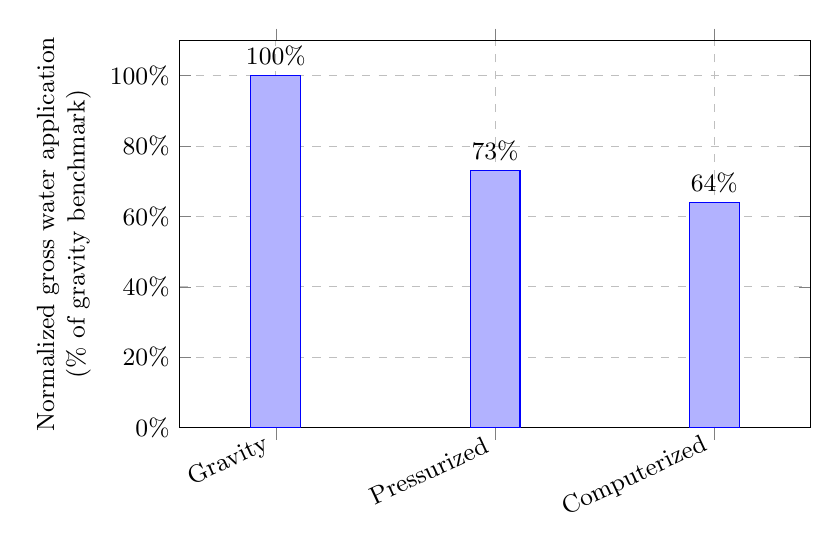
\begin{tikzpicture}
\begin{axis}[
    ybar,
    width=0.72\textwidth,
    height=6.5cm,
    ymin=0,
    ymax=110,
    ylabel={Normalized gross water application\\(\% of gravity benchmark)},
    ylabel style={font=\small,align=center},
    symbolic x coords={Gravity,Pressurized,Computerized},
    xtick=data,
    ytick={0,20,40,60,80,100},
    yticklabel={\pgfmathprintnumber{\tick}\%},
    xticklabel style={rotate=25,anchor=east,font=\small},
    yticklabel style={font=\small},
    nodes near coords={\pgfmathprintnumber{\pgfplotspointmeta}\%},
    nodes near coords style={font=\small,text=black},
    bar width=18pt,
    enlarge x limits=0.22,
    grid=major,
    grid style={dashed}
]
\addplot coordinates {
    (Gravity,100)
    (Pressurized,73)
    (Computerized,64)
};
\end{axis}
\end{tikzpicture}
\end{document}
